%!TEX root = paper.tex
\section{Evaluation}
\label{sec:results}

In this section, we evaluate the accuracy of our BLE fingerprinting
methodology, conduct experiments to study the limitations of RF fingerprinting, and demonstrate the feasibility of deploying the mentioned attack in real-world scenarios. First, to demonstrate the ability of distinguishing even the most similar devices, we evaluate the accuracy of distinguishing 20 transmitters
that are the same make and model (20 for combo chipsets and 20 for BLE-only chipsets) in a
controlled lab environment. This experiment aims to prove that in a controlled environment in which environmental conditions are fairly stable, our fingerprinting methodology is accurate enough to identify the devices even from the same make and model. Second, we experiment the effect of the most influential environmenal parameter, temperature, on the RF fingeerprints. This experiment is in fact, the study of the fundamental limitations of RF fingerprinting. Third, we evaluate how serious these limitations could be in real-world devices by collecting data from a huge pool of people's devices and monitoring the variations of fingerprints of each device. This experiment demonstrates how serious thermal conditions could be in actual devices in use. Fourth, we examine the ability of distinguishing a large number of devices randomly observed in the real world (which people are using). Finally, we evaluate the accuracy and performance of
our attack model and fingerprinting technique when identifying targets in real-world environments.
Specifically, we performed real-world experiments where there are hundreds of
other transmitters that may be confused with the target. These experiments shows this
RF fingerprinting attack could be robust enough to be performed in practice, because
the experiments were performed in uncontrolled environments including coffee
shops, a library, and a food court.


%This is the largest dataset in terms of number of devices used for evaluating
%the RF fingerprinting techniques. 

\subsection{Distinguishing the same make and model}

\begin{figure*}
\centering
%
\begin{minipage}{0.45\textwidth}
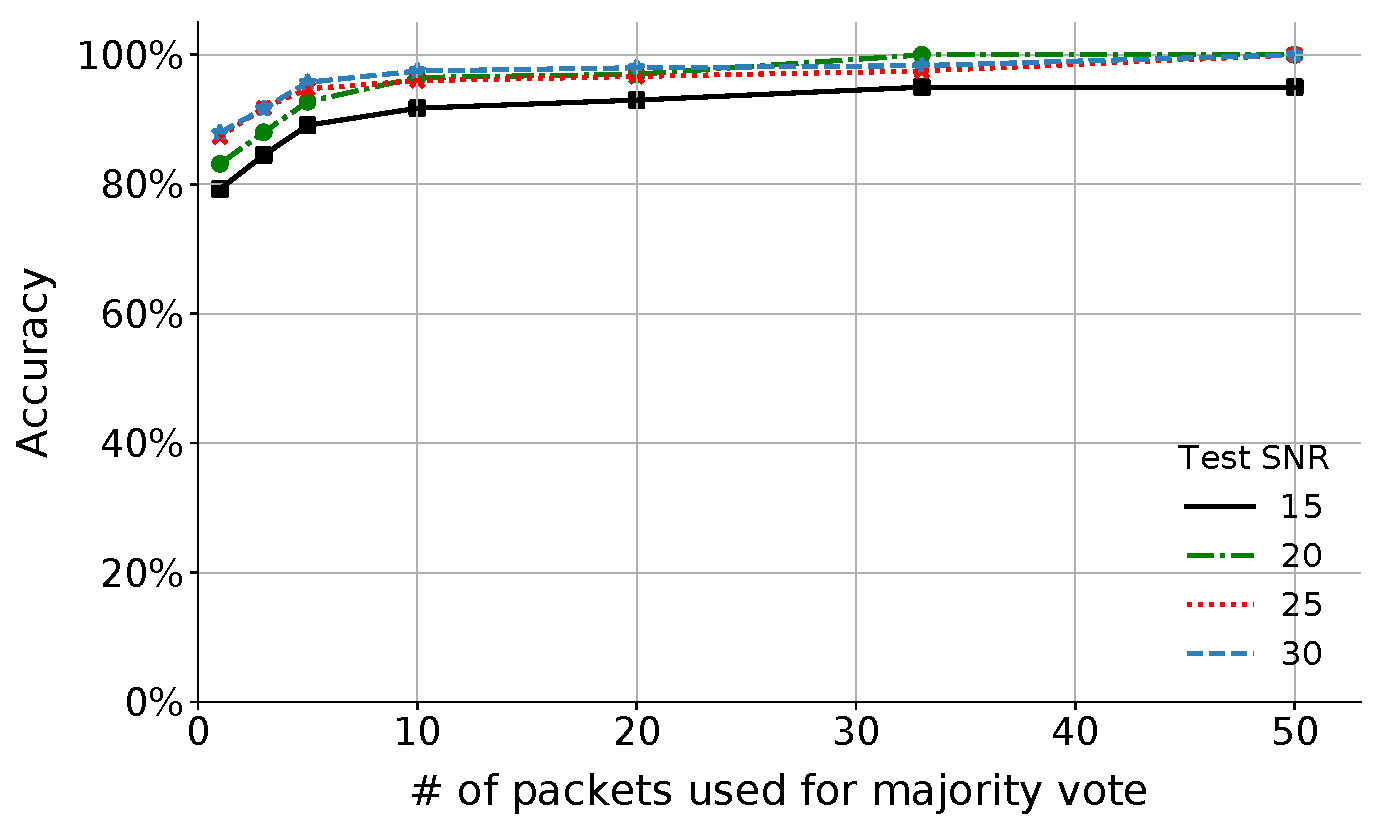
\includegraphics[width=\linewidth]{plots/accuracy_esp.pdf}
\caption{Accuracy of classifying WiFi combo chipsets}
\label{fig:11}
\end{minipage}
%
\hspace{0.04\textwidth}
%
\begin{minipage}{0.45\textwidth}
\centering
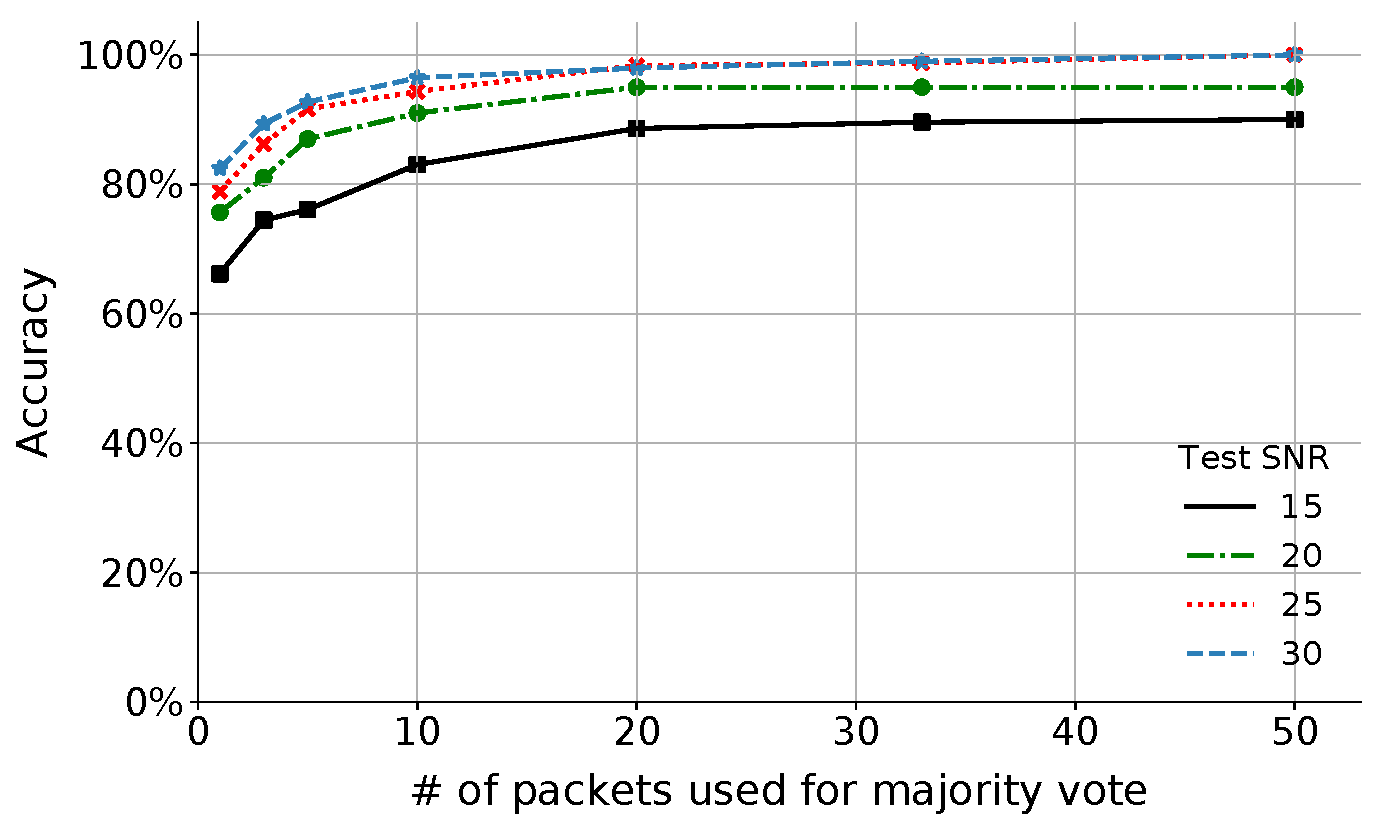
\includegraphics[width=\linewidth]{plots/accuracy_snr2.pdf}
\caption{Accuracy of classifying BLE-only chipsets}
\label{fig:13}
\end{minipage}
%
\end{figure*}

\noindent\textbf{Experiment Setup:} In this section, we seek to answer a basic question: \textit{is it possible to distinguish the most similar BLE devices, that is the devices from the same make and model with a high accuracy even in a controlled lab environment?}. To evaluate the accuracy of distinguishing
transmitters of the same make and model, we purchased 20 devices for each of the two
primary types of BLE chipsets (described in Section~\ref{sec:background}). For
the WiFi/BLE combo chipset we used the popular ESP32 chipset, and for the
BLE-only we used Texas Instrument's popular CC2640 BLE chipset. We set these
devices to transmit BLE advertisements and captured 100 training packets from
the ESP32, and 1000 training packets from the CC2640. We captured these signals
with a USRP N210 Software Defined Radio with a 120~MHz RF frontend. Capturing all 
three of the advertisement channels at once was possible because we used the SparSDR~\cite{sparsdr}
receiver.
All of our captures were at a high SNR (50~dB) so that we could artificially add AWGN noise to in
MATLAB. The SNR range for each packet after adding the noise resulted in 10--30
dB of SNR, a typical range that an attacker would see in the wild.  Finally, we
classified each of the 20 devices for each chipset using the ML-based
fingerprinting algorithm described in the prior section. We used a separate test packet capture to evaluate the accuracy of
distinguishing the devices. In addition, to ensure there was no bias to the
results for SNRs that we trained on, for each SNR we evaluated during the test, we excluded that
SNR from the training data for that experiment. For instance, if the test SNR is 20 dB, the SNR values during training are $\{10,15,25,30\}$.

%The SNR in this experiment is about 50 dB.  For instance, if the test SNR is 20 dB,
%the SNR values during training are $\{10,15,25,30\}$.\\ As an instance of
%IQ-based architecture, we classify 20 ESP32 chipsets.
%since classifying similar devices is harder than different devices.



%Fig. 11 - Robustness of Gradient Descent imperfection estimation under different SNR values - SNR of test data and train data is different

%Fig. 12 - Robustness of Histogram under different SNR values - SNR of test data and train data is different

\subsubsection*{Results}

As mentioned earlier, to demonstrate the robustness of our algorithm under different SNR values, we use different SNR values during training and test. Figures~\ref{fig:11} and~\ref{fig:13} show the test accuracy of classifying the
devices compared to the number of packets used to decide on the classification for different test SNR values.
It is important to compare with the number of packets because obtaining more
packets means that the target must be seen by the attacker for a longer period
of time. To decide the identity of a transmitter upon classifying multiple
packets from it, we applied simple majority voting mechanism. Overall, the
WiFi/BLE combo chips (Figure~\ref{fig:11}) were easier to classify than the
BLE-only chips (Figure~\ref{fig:13}). This is a positive result because we see
far more WiFi/BLE combo devices in the wild (e.g., iPhone) than BLE devices,
and this indicates that the \mbox{I/Q}-based fingerprinting mechanism can
manage to distinguish between these devices. Also, we observe that both types
of devices can be distinguished with close to 100\% accuracy at a high SNR of
25~dB. For both types of devices, at least 20 packets are needed to accurately
classify the devices. These packets can be obtained in less than a minute from
most BLE advertising devices. \textit{This indicates that once the device is fingerprinted, we can distinguish even the devices from the same make and model accurately.}

%\begin{minipage}{0.30\textwidth}
\begin{figure}
\centering
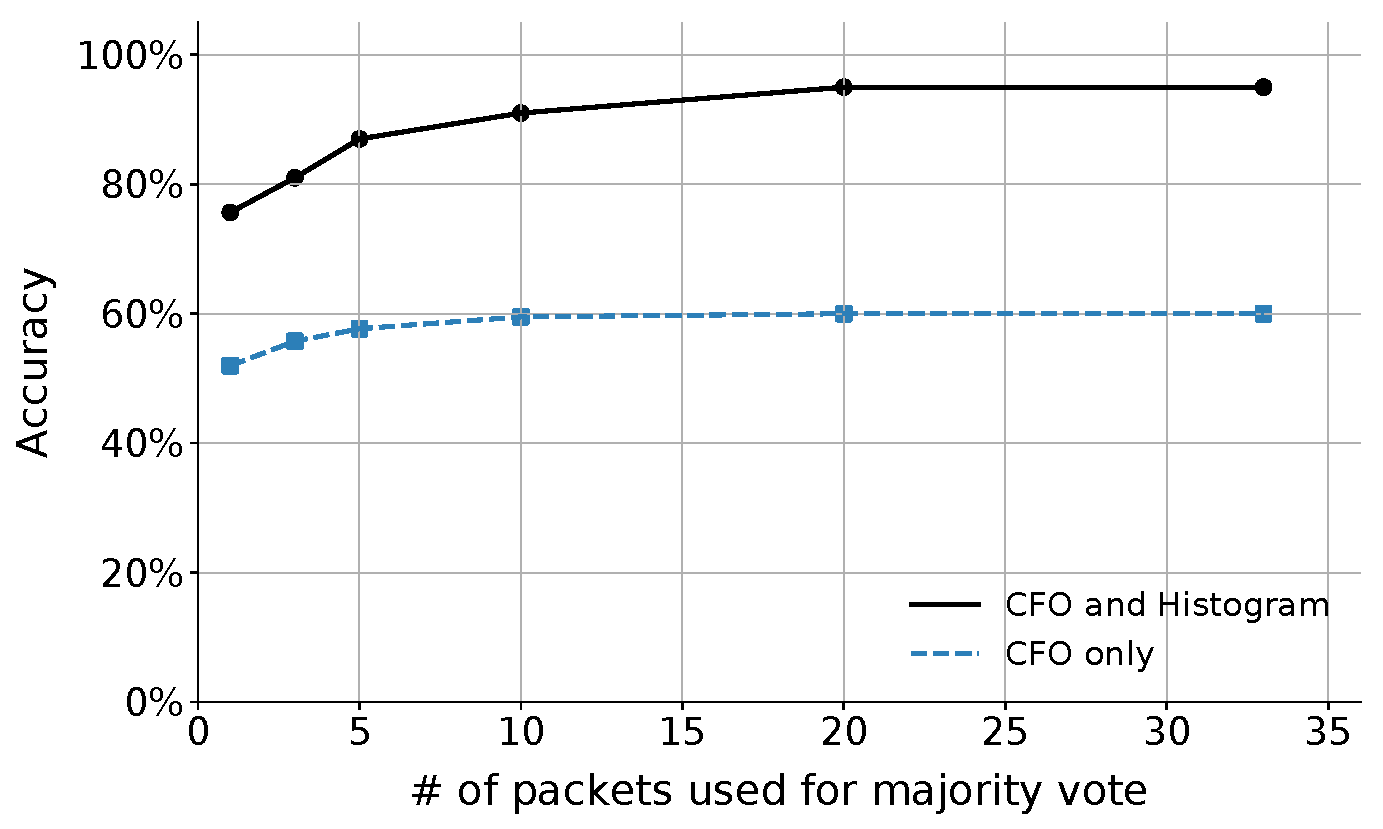
\includegraphics[width=\linewidth]{plots/accuracy_cfo2.pdf}
\caption{Improvement in classification accuracy of BLE-only chipsets from freq. dev. histogram (SNR 20~dB)}
\label{fig:12}
\end{figure}

For the BLE-only devices, we also evaluated the improvement in accuracy
provided by our new fingerprinting technique---the histogram of frequency
deviation.  Figure~\ref{fig:12}, shows the accuracy with CFO alone, and with
CFO combined with the frequency deviation histogram.  We see that although
CFO is somewhat useful on its own, it can only distinguish about half of the
devices. Combining CFO and the histogram is critical to reaching over 90\%
accuracy.


% AARON REMOVED THIS BECAUSE HE HAS NO IDEA WHAT IT IS TALKING ABOUT
%\begin{comment}
As a side note, it's worth mentioning that we use the CNN trained on these 20
TI chipsets as a pre-trained model for the rest of experiments, i.e. we freeze
the convolutional layers and re-train the dense layers for the rest of
experiments to extract features from Histogram. Note that in the following
experiments, we use the data from real people's devices and we do not use these
TI chipsets in any of the following experiments. Therefore, using the CNN as a
pre-trained model does not affect the fairness of the results. The reason for
doing this, is having the flexibility to train the network with less training
data as we do not need to train the network from scratch and have a warm weight initialization.
%\end{comment}



%accuracy of classification for each packet, one important factor in
%identifying the victim is whether by getting more packets from his temporary
%MAC address, we are able to identify him accurately. Therefore, we show the
%accuracy of classification versus the number of packets that we get from a
%device during the test.

\subsection{Thermal effects on RF fingerprints}
RF fingerprints are caused by the imperfections in the analog circuit of the device and thermal conditions may affect the analog circuit inside the device. Consequently, thermal variations may affect the fingerprint of a device and make it no longer identifiable. For instance, crystal oscillators behave differently in different temperatures and varying the temperature can change the error in the frequency they intend to generate (i.e. CFO). Generally, there are two factors that can change the thermal conditions of the circuit: ambient temperature and phone activity. Significant ambient temperature variations can change the internal temperature of the phone and increasing the phone's workload can make the internal phone components warm. In this section, we conduct experiments to evaluate how much thermal conditions can affect RF fingerprints. To the best of our knowledge, this is the first paper to quantify the effects of thermal conditions on the RF fingerprints.

\subsubsection*{Device Activity}
Increasing the device wokload can warm up he internal circuit of the device. For instance, playing a high quality game or video on a phone will consume more power and consequently, the temperature of the internal circuit of the phone will increase. This thermal variation of the circuit can potentially affect the RF fingerprints. In this section, we conduct experiments to demonstrate the effects of differentt workloads on the internal temperature of the phone and RF fingerprints (CFO and IQ offset).
\todo{Hadi: temperature results for different phone workloads} 

\subsubsection*{Ambient temperature}
Other than the device activity, ambient temperature may also change the circuit temperature. However, slight ambient ttemperature variations cannot affect the internal phone temperature. In this section, we seek to figure out how much ambient temperature variation can affect the internal circuit temperature and RF fingerprints considerably. 
\todo{Hadi: temperature results for different ambient temperature. how much ambient temperature changes internal temperature and CFO/IQ}

\subsubsection*{Field data}

\todo{Hadi: Graphs for cfo variations for 200 devices}  

\subsection{Distinguishing devices in the wild}
\label{sec:results:field}

\todo{Hadi: Add specific details about environmental conditions when we were collecting the data (how we the place we collected data, temperature, distance, etc)}
\noindent\textbf{Experiment Setup:}
%
In this experiment, we used the same setup as the previous experiment and collected
	BLE advertisements from hundreds of devices in crowded environments such as
	coffee shops, a library, and a food court. In each of these locations we collected
	advertisements for $\sim$20 minutes.
%
Even though we were analyzing captures from real-world devices, we were careful
	not to analyze the content of the packets we captured: we only analyzed the
	physical layer properties to perform our fingerprinting evaluation. Moreover,
	we did not have any way of correlating a device's MAC address with the owner
	of the device. 
	%because many devices randomize their MAC address. 
	As an
	additional level of protection, we did not analyze devices by their MAC
	address, instead we used these MAC addresses to compute a serial number in order to use as labels, and
	we only processed the data based on these serial numbers.
 
One complication when running this uncontrolled experiment was that the MAC
	address of these devices may change over due to MAC address randomization. This could 
	skew our results toward thinking our fingerprinting method has
	problems distinguishing real-world devices while they are in fact, randomized MAC addresses from the same device.
	%
	To mitigate this
	problem, for the data at a single location, we only consider devices
	that we have observed concurrently with other devices. In fact, we obtained the largest subset of MAC addresses among which any pair have been observered concurrently. This will ensure that the MAC addresses that we considered are presenting different devices.
	%
	This reduced our data set by about half of the devices we observed in the wild, possibly indicating that we observed
	one MAC address change cycle on average during our experiments..

This field experiment persues two major goals. First of all, we want to
evaluate the performance of our fiingerpriting algorithm in the real-world
environment. Second, we aim to figure out the chance that two random devices in the world being
confused with each other which eventually leads to miscalssifying the targets
as non-target devices and vice-versa. This dataset provides a realistic evaluation on the two mentioned goals as it
is fairly large and is collected from actual devices in use which provides a
realistic estimation of the distribution of the devices that people are using.

\begin{comment}
    we classify the packets from different devices at that location. Upon the event of "device confusion" of two device (later we will define our "device confusion" metric), we consider three scenarios:
    \begin{itemize}

    \item If we saw that MAC address at the same time, the confusion is valid and we consider these two MAC addresses as 2 different devices.
    \item If we saw the second MAC address after the first MAC address more than 200 received packet apart (from any device in the environment), the confusion is valid and we consider these two MAC addresses as 2 different devices.
    \item If we saw the second MAC address after the first MAC address less than 200 received packet apart (from any device in the environment), the confusion is invalid and we consider these two MAC addresses from the same device which has randomized its MAC address. Then we assume the same label for these 2 MAC addresses.
    \end{itemize}
    Although this does not rule out the possibility of considering the same device with two MAC addresses as 2 different devices, it reduces the chance of this event. \\
\end{comment}

\subsubsection*{Results}
\todo{Hadi: add a figure like figure 4 for the devices in the wild}

\begin{figure}
    \centering
    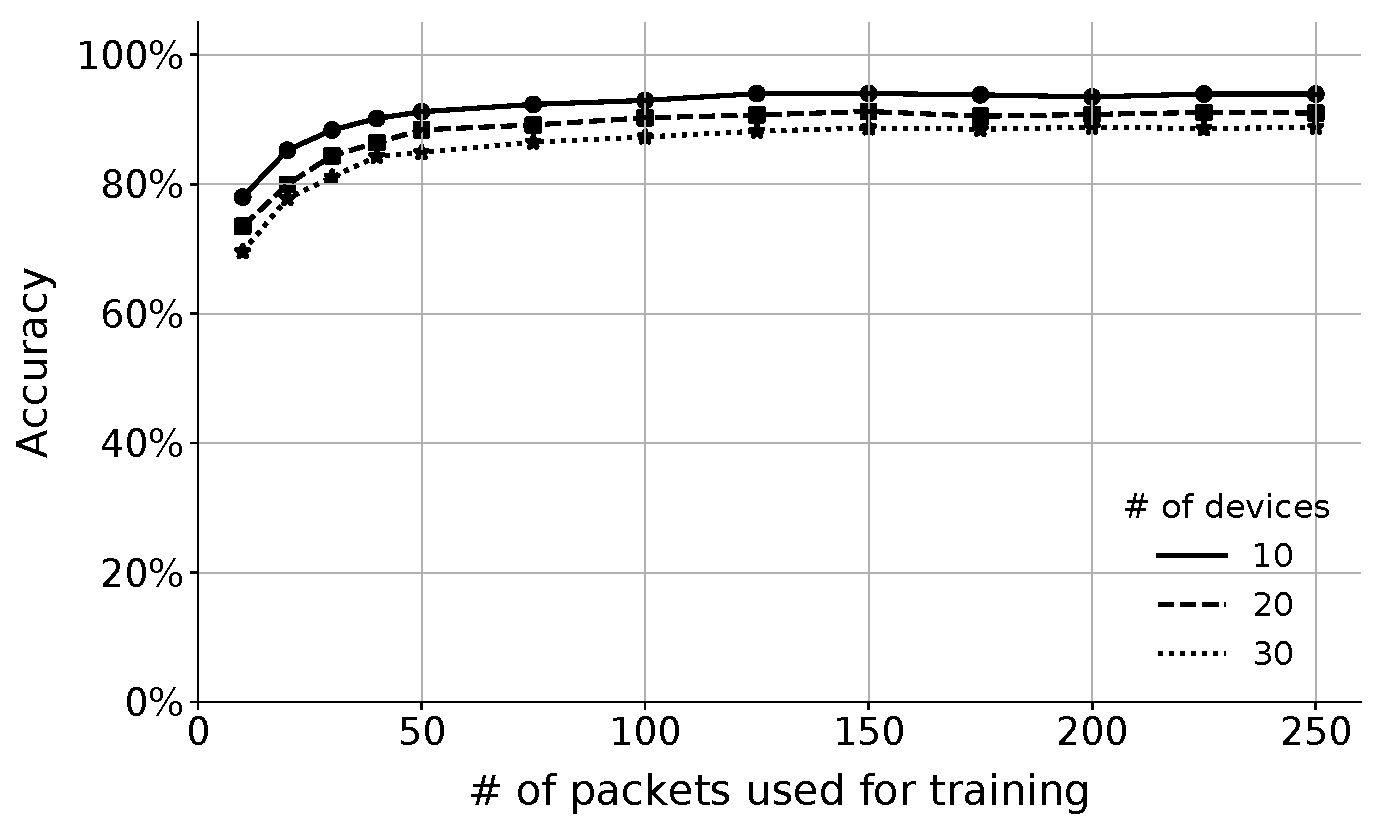
\includegraphics[width = \linewidth]{plots/learning_curve.pdf}
    \caption{Learning curve - Test Accuracy vs the number of training samples per devices}
    \label{fig:14}
\end{figure}

First, we determine the number of packets we need from a device in
order to be able to fingerprint and distinguish that with a decent accuracy. To
do so, we observe the test accuracy by increasing the number of training
examples per device. Figure~\ref{fig:14} shows the test accuracy as the number
of training example per device increases, for the classification of 10, 20 and
30 random devices from the field experiments. For each of the sets of devices,
we randomly picked the devices from the set of all devices 100 times and
averaged the accuracy across these 100 runs. This figure shows 100 packets per
device is sufficient for classification as the accuracy does not increase
significantly for more than 100 packets. However, to have a larger set of
devices to analyze, we sacrifice the accuracy a little bit and consider all the
devices (i.e, unique MAC addresses after dealing with MAC address changes from
1 device as discussed above) from which we got more than 60 packets (50 for
training or "fingerprinting stage" and 10 for test or "identification stage").
After filtering out these devices, we have 220 different devices to analyze.

\begin{figure}
    \centering
    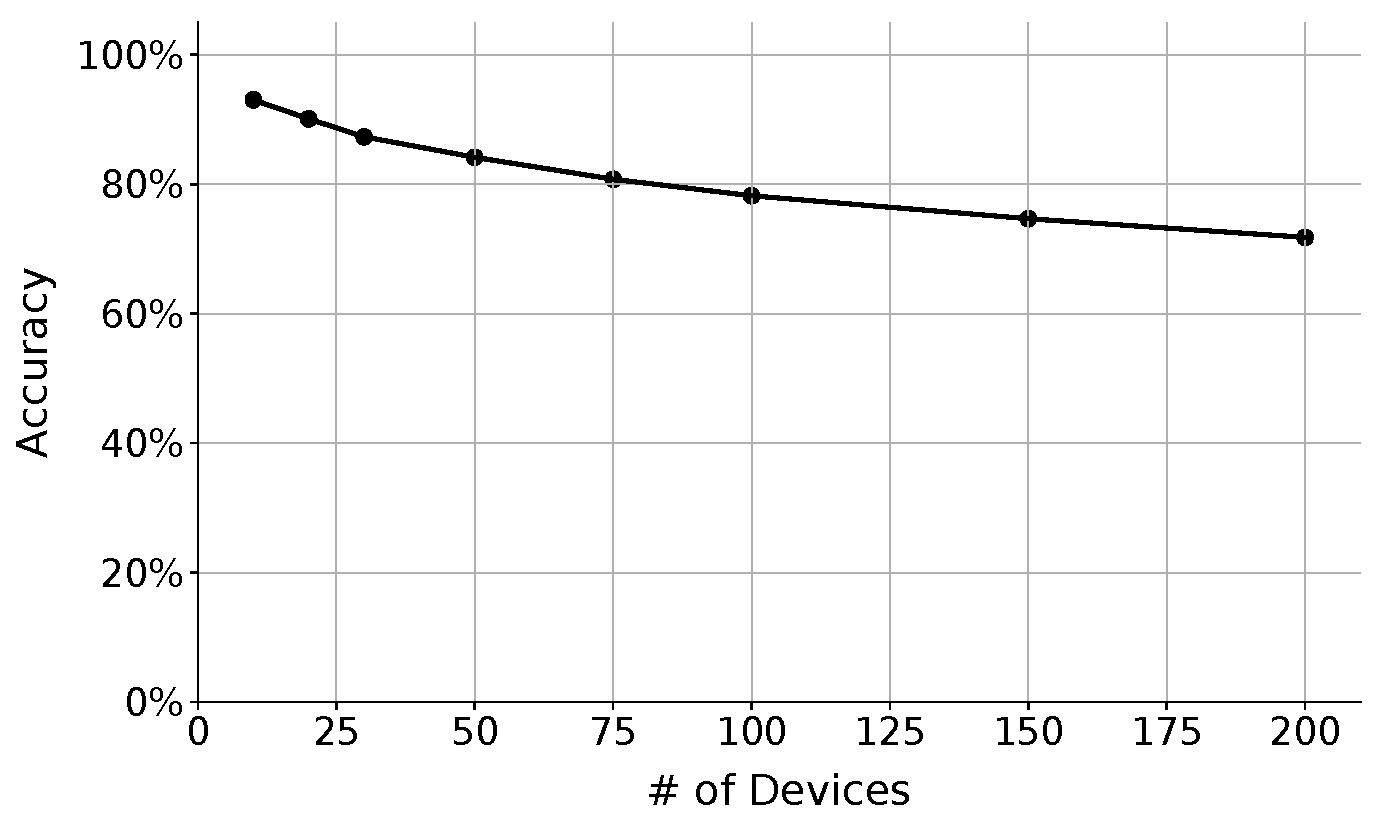
\includegraphics[width = \linewidth]{plots/accuracy_device.pdf}
    \caption{Accuracy of classifying a single packet for different number trained devices}
    \label{fig:15}
\end{figure}



Next, we analyze the accuracy of classifying a single packet correctly as we
increase the number of devices. For each set of $n$ devices to be classified,
we randomly pick $n$ devices from the set of 220 devices and compute the
classification accuracy.  We repeat this process 100 times and take the average
accuracy across these 100 experiments. Figure~\ref{fig:15} shows this
classification accuracy for different number of devices. The accuracy drops off
steadily as we increase the number of devices, but the drop is not linear.


\begin{figure}
    \centering
    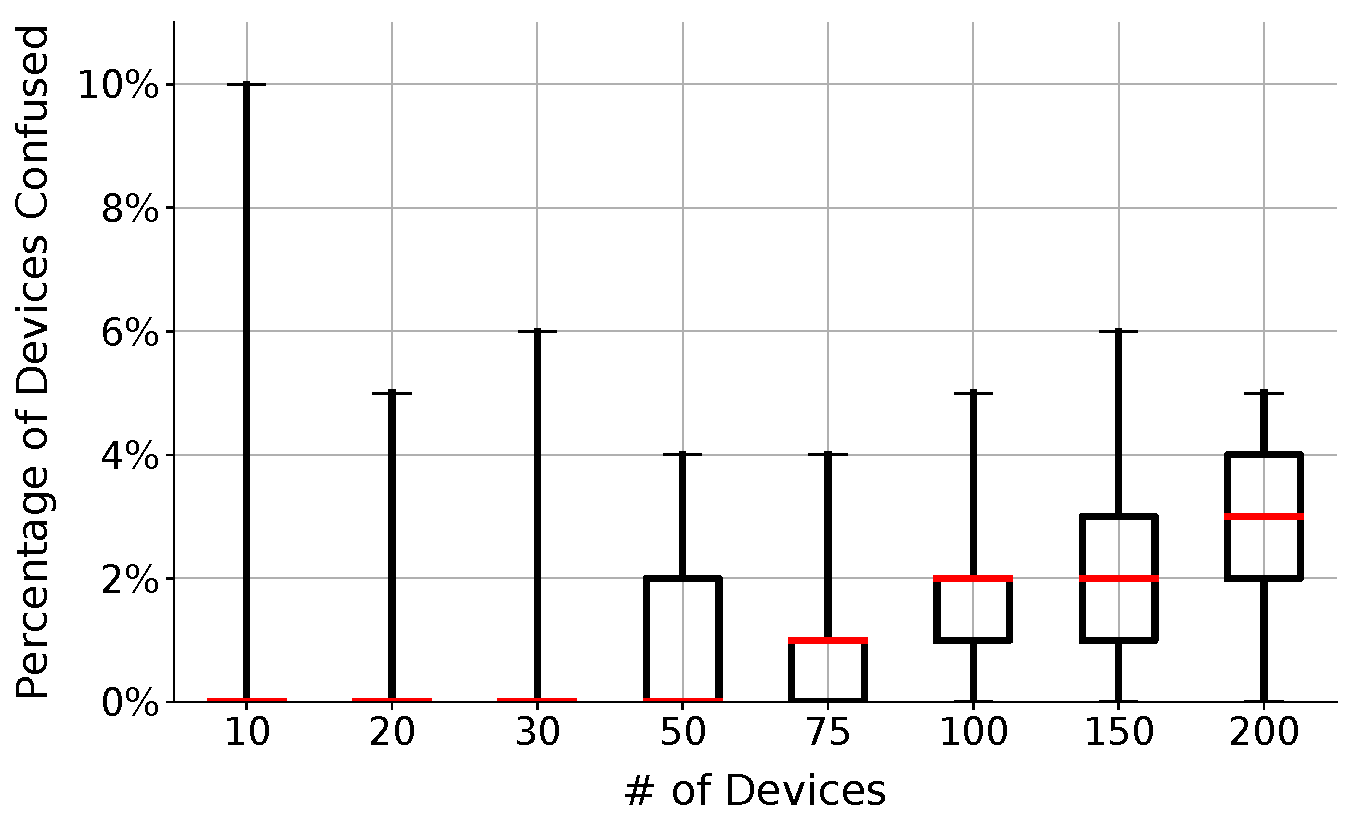
\includegraphics[width = \linewidth]{plots/box_whisker.pdf}
    \caption{Number of device confusions for sets of different number of devices}
    \label{fig:16}
\end{figure}


We also evaluate the chance that we confuse a device with another device.  The
box and whisker plot of the percentage of device confusions is shown in
Figure~\ref{fig:16} for different number of device classes. The box shows 25
and 75 percent and the line shows the maximum and minimum.  To analyze the chance of confusing the devices, we followed the following procedure. Assume we receive
$k$ packets from a single MAC address during the identification stage. It is
possible that we classify these packets as different devices. However, we know
that they are coming from a single device since they share the same MAC address.
Therefore, a simple way to decide about a single class (device) to which these
packets are assigned is taking a majority vote across the classes that these
$k$ packets are classified as. In other words, if we have $n$ classes of
devices labeled as $\{c_1,c_2,c_3,...,c_n\}$, and these packets are classified
as $\{c_1',c_2',c_3',...,c_k'\}$, then the corresponding MAC address is
assigned to class $c_i = mode \{c_1',c_2',c_3',...,c_k'\}$ where $i \in
\{c_1,c_2,c_3,...,c_n\}$. According to this, the event that we confuse the
device $A$ with another device after receiving $k$ packets from device $A$
(which now has a different MAC address that we don't know. However, the MAC
addresses of all of these $k$ packets are the same) will happen when the
majority vote between these $k$ packets is a class other than $c_A$. We call
this event a "device confusion". We also consider  the case of a tie between
the true class and another class as a device confusion. Now, we repeat the same
analyses as we did for calculating the accuracy of classifying different number
of devices (we repeat 100 times for each number of device classes). This time,
instead of accuracy, we count the number of device confusions when we have
$k=10$ packets from each device during the identification stage and 50 packets
during the fingerprinting (training) stage. 

The choice of 50 packets for training has been explained according to Figure~\ref{fig:14} before. The reason for choosing 10 packets for taking majority vote during the identification stage (test stage), is that this is the minimum number of packets which is needed from a device in order to be identified reliably. As we get more packets, we do indeed improve our ability to identify the device. However, in our experiments we found that beyond using 10 packets for identification, the accuracy of our decision doesn’t improve significantly.



\subsection{End-to-end Attack Evaluation}
\label{sec:results:attack}
\noindent\textbf{Experiment Setup:}
To demonstrate the feasibility of our attack model in the real-world setting, we
considered 15 volunteer's devices as targets (8 iPhones, 3 Apple watches, 1
FitBit, 1 Bose headphones, 1 Thinkpad laptop, 1 MacBook laptop). We fingerprinted
these devices in a library where exists many people and checked the MAC address
of our devices to use as labels. Then we treated the non-target devices
(devices of random people in the library) as a separate class of device. Then
we trained our model on these $15+1$ class of devices. We used only 100 packets
from each of the targets which is easily available in less than a minute for
most of devices. During the identification, if some device was classified as
the 16th class, then it is none of the targets.
%
One week later, we took 5 of the
targets (1 from each kind of device except the apple watch) to a food court. We
captured the signal from our target devices as well as other devices in the
food court. We checked the MAC address of the targets manually as ground truth.

\subsubsection*{Results}

The two questions from this experiment are: what is the probability that we
mistakenly classify a non-target device as one of the targets (false positive
rate)? and what is the probability that one of the targets is in the crowd but
we think it is not (false negative rate)? We calculate the false positive 
and negative rate based on the number of devices that were confused when
we take the majority vote of 10 packet classifications (the choice of 10 packet is made according to subsection~\ref{sec:results:field}). 

In addition to our targets, we observed 40 devices in the food court. Using the model that was trained on library data, the false positive of this experiment was 2.5\%, meaning we thought 2.5\%
percent of the non-target devices are one of the targets, and the false
negative was 0\% meaning we detected all target properly.
%
Next, we collected data from 130 devices in 5 different coffee shops where non
of the targets were present. The goal of this experiment was getting a
realistic estimate of false positive rate with having more non-target devices around since these many non-target devices observed in several locations can approximates the distribution of devices that we may see in other places that one may run the attack as well. The false positive rate in this
experiment was 2.3\% by using the same model trained on library data. This demonstrates the feasibility of deploying such an attack in real-worl environment. In fact, we were able to identify the targets 1 week later in a completely new place.


\subsection{A Positive Use Case: Defense Against Re-broadcasting Attack}